\documentclass[12pt]{article}

\usepackage{sbc-template}

\usepackage{graphicx,url}

\usepackage[brazil]{babel}   
%\usepackage[latin1]{inputenc}  
\usepackage[utf8]{inputenc}  
% UTF-8 encoding is recommended by ShareLaTex

     
\sloppy

\title{Implementação e Avaliação de um Mecanismo de Detecção de Anomalias em uma Ferramenta Smart Grid}

\author{Luiza S. Eitelvein\inst{1}, Alexandre G. Wermann\inst{1}, Luciano P. Gaspary\inst{1},\\
 Marinho P. Barcellos\inst{1}, Alberto E. Shaeffer-Filho\inst{1}}


\address{Instituto de Informática -- Universidade Federal do Rio Grande do Sul
  (UFRGS)\\
  Caixa Postal 15.064 -- 91.501-970 -- Porto Alegre -- RS -- Brazil
  \email{\{lseitelvein,agwermann,paschoal,marinho,alberto\}@inf.ufrgs.br}
}

\begin{document} 

\maketitle

\begin{abstract}
Smart grids combine ICT based communication networks and electric grids with the goal of providing a more efficient and automatized energy distribution, besides allowing the introduction of distributed energy production sources, including renewable sources. SCADA systems, responsible for controlling devices and collecting information in the smart grid, allow real time monitoring of the energy production and consumption information. However, these systems are vulnerable to cyber attacks, among other threats. In this work, we present an Anomaly Detection System, based on network traffic classification, developed for the ASTORIA toolset, which allows the simulation of smart grid environments and the definition of attacks. The anomaly detection in the network traffic is performed by the OCSVM algorithm, which was chosen because it allows one class classification, only with knowledge of normal network traffic data. Through experiments we performed, using simulation scenarios containing DoS attacks and anomalies in the size of the measured packets, we verified that the proposed system is capable of identifying anomalies in the network traffic with an accuracy greater than 97\%, correctly classifying all the occurrences of anomalous traffic and presenting a false alarm rate of up to 3\%.
\end{abstract}

\begin{resumo}
Smart grids combinam redes de comunicação baseadas em ICT e redes elétricas com o objetivo de fornecer uma distribuição de energia mais eficiente e automatizada, além de permitir a introdução de fontes de produção de energia distribuídas, incluindo fontes renováveis. Sistemas SCADA, responsáveis pelo controle de dispositivos e coleta de informações ao longo de todo o smart grid, permitem o monitoramento em tempo real das informações de produção e consumo de energia. Todavia, esses sistemas estão vulneráveis a ataques cibernéticos, entre outras ameaças. Neste trabalho, apresentamos um Sistema de Detecção de Anomalias, baseado na classificação do tráfego de rede, desenvolvido para a ferramenta ASTORIA, que permite a simulação de ambientes smart grid e a definição de ataques. A detecção de anomalias no tráfego é realizada através do algoritmo OCSVM, escolhido por permitir a classificação em classe única, com conhecimento apenas do tráfego normal da rede. Através dos experimentos realizados, com simulações de cenários de ataques DoS e anomalias no tamanho dos pacotes medidos, verificamos que o sistema proposto é capaz de identificar anomalias no tráfego da rede com uma acurácia superior a 97\%, classificando corretamente todas as ocorrências de tráfego anômalo e apresentando uma taxa de até 3\% de alarmes falsos.
\end{resumo}

\section{Introdução}

	Smart grids são sistemas modernos de distribuição de energia, formados por redes elétricas tradicionais em conjunto com Sistemas de Controle de Supervisão e Aquisição de Dados – \textit{Supervisory Control and Data Acquisition (SCADA)}, a fim de prover maior automação e segurança à rede, além  de uma distribuição de energia mais eficiente e confiável \cite{2013survey}. A agregação de capacidade computacional à rede elétrica, em conjunto com o fluxo bidirecional de energia e de informação, e com a instalação de infraestruturas avançadas de medição e controle,  possibilitam diversos avanços em direção ao consumo e distribuição mais eficientes de energia elétrica.  Smart grids podem receber energia de fontes distribuídas, incluindo fontes renováveis e pequenos produtores. Também é possível fornecer aos consumidores informações sobre como e quando seu consumo de energia é mais elevado, e oferer opções de gerenciamento de consumo através do controle de dispositivos inteligentes presentes nas residências \cite{harb2013communication}.

No entanto, a utilização de uma rede de comunicação baseada em Tecnologia de Informação e Comunicação - \emph{Infomation and Communication Technology (ICT)} na infraestrutura do smart grid introduz a vulnerabilidade à ataques cibernéticos \cite{li2012securing}. É imprescindível que um smart grid seja seguro e robusto contra ataques, pois, sendo uma estrutura crítica, a interrupção do serviço pode cessar o fornecimento de energia elétrica à uma região inteira \cite{massoud2005toward}. Embora existam diversas tecnologias voltadas à segurança de redes baseadas em ICT, elas não são adequadas para garantir a segurança dos componentes de um smart grid \cite{carcano2011multidim}. Dessa forma, é de grande importância desenvolver novos mecanismos de segurança projetados especificamente para sistemas SCADA e para os demais componentes de um smart grid.

O objetivo deste trabalho consiste em desenvolver um sistema de detecção de anomalias para uma ferramenta que simule o ambiente de execução de um smart grid utilizando um algoritmo de classificação do tráfego da rede de comunicação. A partir do uso de uma ferramenta para simular o tráfego de comunicação de um smart grid, o sistema de detecção deve ser capaz de acessar os fluxos de dados entre os componentes da rede e utilizar as informações obtidas para detectar a existência de ataques ao sistema.

O sistema de detecção proposto neste trabalho utiliza a ferramenta ASTORIA \cite{wermann2015astoria} para a simulação de um ambiente smart grid. As informações do tráfego da rede de comunicação são utilizadas pelo mecanismo de detecção para detectar anomalias no sistema, que podem indicar a ocorrência de um ataque. A detecção de anomalias é realizada através do \emph{One-Class Support Vecotr Machine (OCSVM)}, um algoritmo de Aprendizado de Máquina voltado para a classificação de dados em uma única classe, utilizando atributos derivados do tamanho dos pacotes e da frequência dos pacotes entre os dispositivos da simulação. A avaliação do sistema de detecção desenvolvido é feita através de experimentos com simulações de cenários com a ocorrência de ataques de Negação de Serviço - \emph{Denial of Service (DoS)} e anomalias no tamanho dos pacotes de rede analisados.

No Seção \ref{stateofart}, é apresentada a fundamentação teórica, descrevendo a arquitetura dos smart grids e os mecanismos de detecção de anomalias. A Seção \ref{project} apresenta o sistema de detecção de anomalias proposto, descrevendo o framework ASTORIA, utilizado para a simulação do ambiente smart grid, o algoritmo \emph{One-Class Support Vector Machine}, utilizado para a classificação de tráfego, e o projeto do sistema. A implementação do protótipo do mecanismo de detecção é descrita na Seção \ref{secimpl}, juntamente com os experimentos realizados para a avaliação do mecanismo e a análise dos resultados obtidos. A Seção \ref{related} descreve trabalhos relacionados. Finalmente, a Seção \ref{capconcl} apresenta a conclusão, o resumo das contribuições e trabalhos futuros.

\section{Fundamentação Teórica}
\label{stateofart}
Nesta seção, será estabelecida a fundamentação teórica dos tópicos abordados neste trabalho, afim de apresentar o estado da arte dos conceitos e tecnologias que serão utilizados. A seção \ref{secarq} introduz a arquitetura dos smart grids, e a Seção \ref{mldetection} aborda os mecanismos de detecção de anomalias.

\subsection{Arquitetura dos Smart Grids}
\label{secarq}

	Um smart grid é composto por duas estruturas principais: uma rede elétrica e uma rede de comunicação. A distribuição de energia é feita por redes elétricas tradicionais, operando nos dois sentidos. A rede de comunicação é formada por um Sistema de Controle de Supervisão e Aquisição de Dados – \textit{Supervisory Control and Data Acquisition (SCADA)}.
A produção de energia em um smart grid está distribuída em diversas fontes, que incluem usinas fixas e móveis e microprodutores. A energia elétrica é transportada das usinas de geração até as subestações de transmissão através de cabos de alta tensão, e então é transmitida, assim como a energia de outras fontes diversas, até as subestações de distribuição através de linhas de tensão variada. A partir das subestações de distribuição, finalmente, a energia é distribuída para consumo \cite{harb2013communication}. Sensores inteligentes instalados ao longo de toda a extensão da rede coletam, em tempo real, informações detalhadas sobre o consumo de energia, formando uma AMI \cite{2013survey}.

O sistema SCADA realiza, de forma automatizada, o controle e monitoramento da rede. De maneira geral, os componentes básicos que constituem uma infraestrutura SCADA são Dispositivos de Campo (DCs), Unidades Terminais Remotas - \emph{Remote Terminal Units (RTUs)} e Unidades Terminais Mestres - \emph{Master Terminal Units (MTUs)}.

\begin{itemize}

\item{DCs}: Geralmente constituídos por RTUs ou Controladores Lógicos Programáveis - Programmable Logic Controllers (PLCs), DCs se conectam aos sensores e aos Dispositivos Eletrônicos Inteligentes (DEIs) para receber informações sobre produção e consumo de energia e enviar sinais de controle provenientes do sistema.
\item{RTUs}: RTUs  coletam dados de todos os DCs de uma determinada área e os encaminham para a MTU responsável pela região.
\item{MTUs}: Os dados de todos os DCs de uma determinada região são enviados, através das RTUs, para uma MTU. A MTU, por sua vez, encaminha esses dados para um centro de controle regional, onde eles são monitorados e analisados.
\end{itemize}
A figura \ref{fig:sgarchitecture} ilustra a arquitetura genérica da infraestrutura de um smart grid.

\begin{figure}[h]
   \caption{Arquitetura de um smart grid}
   \begin{center}
       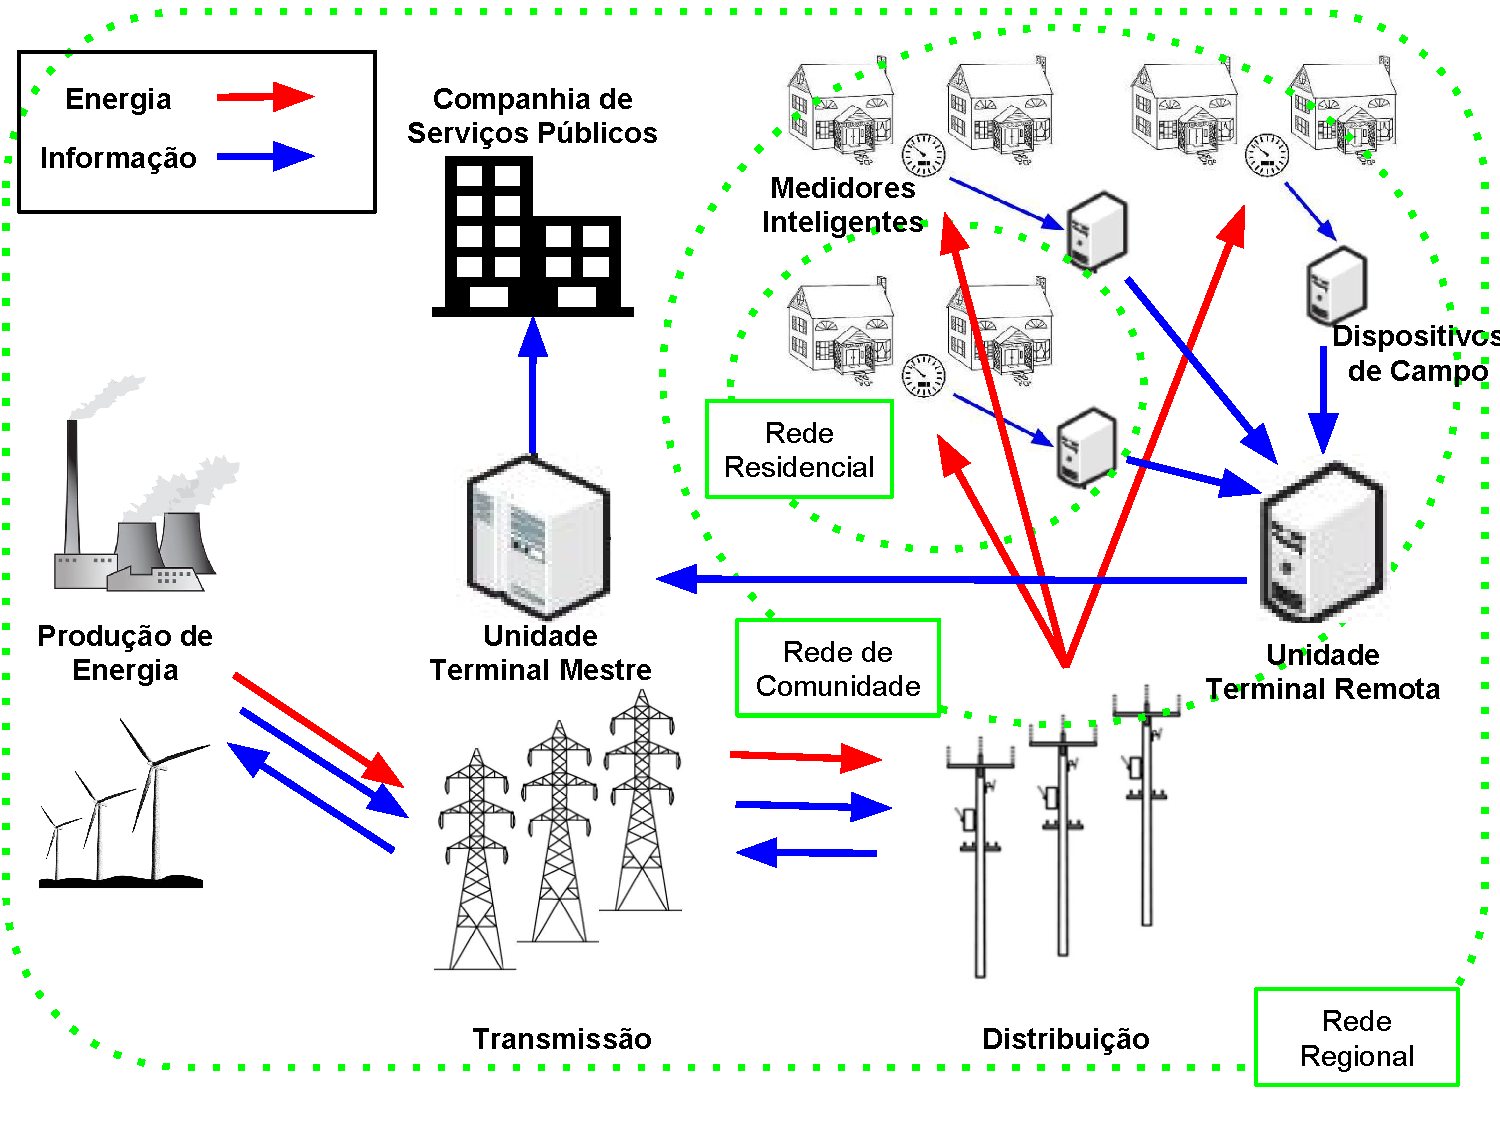
\includegraphics[width=30em]{smart_grid_arch}
   \end{center}
   \label{fig:sgarchitecture}
\end{figure}

A comunicação entre os dispositivos do sistema SCADA é realizada por um protocolo de comunicação. Entre os diversos protocolos disponíveis para comunicação em sistemas SCADA, os mais amplamente utilizados são o Modbus e o DNP3, que surgiram como protocolos seriais e foram estendidos para redes TCP/IP \cite{drias2015taxonomy}.

\subsection{Detecção de Anomalias}
\label{mldetection}
	Garantir confiabilidade e segurança é um grande desafio no desenvolvimento dos smart grids, pois ataques maliciosos podem ser direcionados tanto à rede elétrica física quanto à rede de comunicação \cite{li2012securing}. Apesar da existência de uma vasta gama de tecnologias de segurança voltadas à ICT, essas medidas de segurança não são capazes de resguardar o sistema contra ataques desenvolvidos para atingir sistemas SCADA, medidores inteligentes e outros componentes do smart grid \cite{carcano2011multidim}. Assim, o desenvolvimento de novos mecanismos para tornar os smart grids mais seguros contra falhas e ataques é de grande importância.
	A detecção de anomalias na rede de um smart grid pode ser realizada através da classificação do tráfego de dados da rede. Algoritmos de Aprendizado de Máquina - \emph{Machine Learning (ML)} têm sido utilizados para a classificação de tráfego de dados por possibilitarem a classificação dos dados através de atributos que podem ser observados externamente, como tamanho dos pacotes e tempo entre a chegada de pacotes, sem a necessidade de inspeção do campo de dados do pacote \cite{nguyen2008survey}. Os algoritmos de ML podem ser classificados em duas categorias:

\begin{itemize}
\item{Aprendizado supervisionado}: No aprendizado supervisionado, o algoritmo é treinado utilizando um conjunto de instâncias já classificadas, rotuladas com classes pré-definidas. O modelo gerado no treinamento é utilizado para classificar um conjunto de instâncias desconhecidas. Existe uma vasta gama de algoritmos de aprendizado supervisionado, um exemplo sendo o algoritmo de classificação \emph{Naive Bayes} \cite{rish2001empirical}.
\item{Aprendizado não supervisionado}: Algoritmos de aprendizado não supervisionado não possuem uma fase de treinamento com classes já definidas. Em vez disso, implementam heurísticas para descobrir padrões entre os dados das instâncias e agrupá-las em \emph{clusters} com características similares. Os grupos podem ser exclusivos, quando uma intância não pode pertencer a mais de um grupo, ou sobrepostos, quando as instâncias podem pertencer a diversos grupos. Os principais métodos de aprendizado não supervisionado são os algoritmos \emph{k-means} \cite{wagstaff2001constrained}, clusterização incremental \cite{ester1998incremental} e clusterização baseada em probabilidade \cite{fraley2002model}.
\end{itemize} 

\section{Sistema de Detecção de Anomalias em uma Ferramenta Smart Grid}
\label{project}
Nesta seção, serão apresentadas a modelagem e as ferramentas utilizadas para o desenvolvimento de um mecanismo de detecção de anomalias para uma ferramenta de simulação de smart grid. A Seção \ref{secastoria} descreve o framework ASTORIA, utilizado para configurar as simulações do ambiente smart grid. A Seção \ref{subsecocsvm} o algoritmo \emph{One-Class Support Vectors Machine}, utilizado para a classificação do tráfego da simulação. A Seção \ref{secsdiast} apresenta a modelagem do mecanismo de detecção proposto e descreve seu funcionamento.

\subsection{Simulação de um smart grid com o Framework ASTORIA}
\label{secastoria}

O Framework ASTORIA, descrito pelos autores em \cite{wermann2015astoria}, permite modelar simulações de ambientes smart grid, definir e executar ataques nesses ambientes e avaliar seus resultados e o comportamento do sistema. A simulação consiste de uma rede de energia elétrica e uma rede de comunicação. A rede de energia elétrica é composta por nodos de geração, consumo e distribuição de energia. A rede de comunicação é composta por sensores, RTUs e MTUs. Cada nodo de produção, distribuição e consumo presente na rede elétrica possui um nodo correspondente na rede de comunicação SCADA. Cada nodo de produção ou consumo está pareado com um sensor SCADA, enquanto os nodos de distribuição de energia estão pareados com as RTUs. As MTUs não possuem nenhum componente respectivo na rede elétrica, por serem um componente exclusivo da estrutura SCADA.

A comunicação entre os componentes SCADA acontece através do protocolo modbus. Cada sensor da rede de comunicação recebe as informações sobre o consumo de energia do nodo da rede elétrica associado a ele. A cada passo de execução, as RTUs enviam requisições para todos os sensores conectados a elas, e os sensores respondem enviando os dados de consumo obtidos. A MTU envia requisições para todas as RTUs, que enviam respostas contendo as informações recolhidas de toda a sua região. A topologia da simulação é definida por um arquivo de configuração em que são instanciados os componentes MTU, RTUs e sensores, e as conexões entre os componentes. Todas as RTUs são conectadas à MTU, e cada RTU possui um conjunto de sensores conectados a ela.

O framework ASTORIA também oferece uma biblioteca de ataques, que podem ser executados sobre a simulação do smart grid. Os ataques podem ser instanciados através de perfis, que permitem a configuração de diferentes tipos de ataques. Os perfis de ataques são compostos pelos parâmetros Tipo de Ataque, Nodo de Origem, Nodo Alvo, Passo de Execução e Tempo de Início, além de uma lista de parâmetros opcionais, como tamanho dos pacotes enviados. O framework implementa um ataque de Negação de Serviço - \emph{Denial of Service (DoS)} e um ataque de Injeção de Software Malicioso. Entretanto, o framework e a biblioteca de ataques são extensíveis, e novos perfis de ataques podem ser definidos e implementados.

\subsection{\emph{One-Class Support Vectors Machine}}
\label{subsecocsvm}

	\emph{One-Class Support Vectors Machine (OCSVM)}, proposto em \cite{scholkopf2001svm}, é um algoritmo de ML de aprendizado supervisionado, e é um caso específico do algoritmo SVM \cite{cortes1995support} para Classificação em Classe Única. Algoritmos de Classificação em Classe Única são treinados para reconhecer apenas uma classe de dados. Todas as instâncias do conjunto de treinamento pertencem a uma única classe e os dados analisados pelo algoritmo são classificados como pertencentes à classe (normais) ou não pertencentes à classe (anômalos). O algoritmo OCSVM é particularmente interessante para a classificação do tráfego em um sistema SCADA, pois o classificador pode ser treinado com um conjunto de dados proveniente do tráfego normal da rede. Assim, não é necessário obter dados de tráfego característicos de ataques cibernéticos à sistemas SCADA, nem classificar exaustivamente todos os tipos de ataques possíveis à rede com instâncias de treinamento.

A tarefa de classificação de dados utilizando o OCSVM consiste nos seguintes passos:
\begin{itemize}
\item{Obtenção do conjunto de treinamento}: Definição de um conjunto de instâncias de treinamento para gerar o modelo de classificação.
\item{Treinamento do algoritmo}: A partir do conjunto de treinamento, o algoritmo gera um modelo de classificação, composto por diversas regras para a classificação das instâncias de dados.
\item{Classificação}: Após o treinamento, o algoritmo é capaz de classificar instâncias desconhecidas, ou seja, que não fazem parte do conjunto de treinamento. O algoritmo utiliza o modelo de classificação, gerado na etapa de treinamento, para identificar as novas instâncias como pertencentes ou não à classe de dados representada.
\end{itemize}

Para a classificação do tráfego de rede, as instâncias representam informações sobre os fluxos da rede. Os fluxos caracterizam cada par de dispositivos presentes na rede que trocam pacotes entre si. Assim, os atributos utilizados nas instâncias consistem em métricas que descrevem o comportamento dos fluxos da rede. Não existe um consenso sobre a quantidade de atributos utilizados na classificação com o OCSVM, pois os resultados obtidos com diferentes conjuntos de atributos têm grande dependência do tipo de informações sendo representadas.

 
\subsection{Projeto do Mecanismo de Detecção de Anomalias para a ferramenta ASTORIA}
\label{secsdiast}
O objetivo da implementação de um mecanismo de detecção de anomalias para a ferramenta ASTORIA é que ele funcione como um mecanismo de segurança do sistema, identificando comportamentos anômalos no tráfego de rede e realizando o registro dos dados do fluxo de rede onde as anomalias foram percebidas. Para tanto, os seguintes requisitos devem ser cumpridos:
\begin{itemize}
\item{} A fim de realizar a análise do tráfego, o mecanismo deve ter acesso às informações de dispositivo de origem, dispositivo de destino e tamanho do pacote dos pacotes da rede durante a simulação, para que os atributos dos fluxos de rede possam ser identificados.
\item{} O mecanismo deve utilizar os dados capturados para realizar a classificação do tráfego em normal ou anômalo durante a simulação, registrando ocorrências de tráfego anômalo.
\item{} O mecanismo deve ser independente da topologia da simulação e dos dados sobre o fluxo de energia trocados pelos componentes.
\end{itemize}

\begin{figure}[h]
   \caption{Arquitetura Conceitual do Sistema de Detecção Proposto}
   \begin{center}
       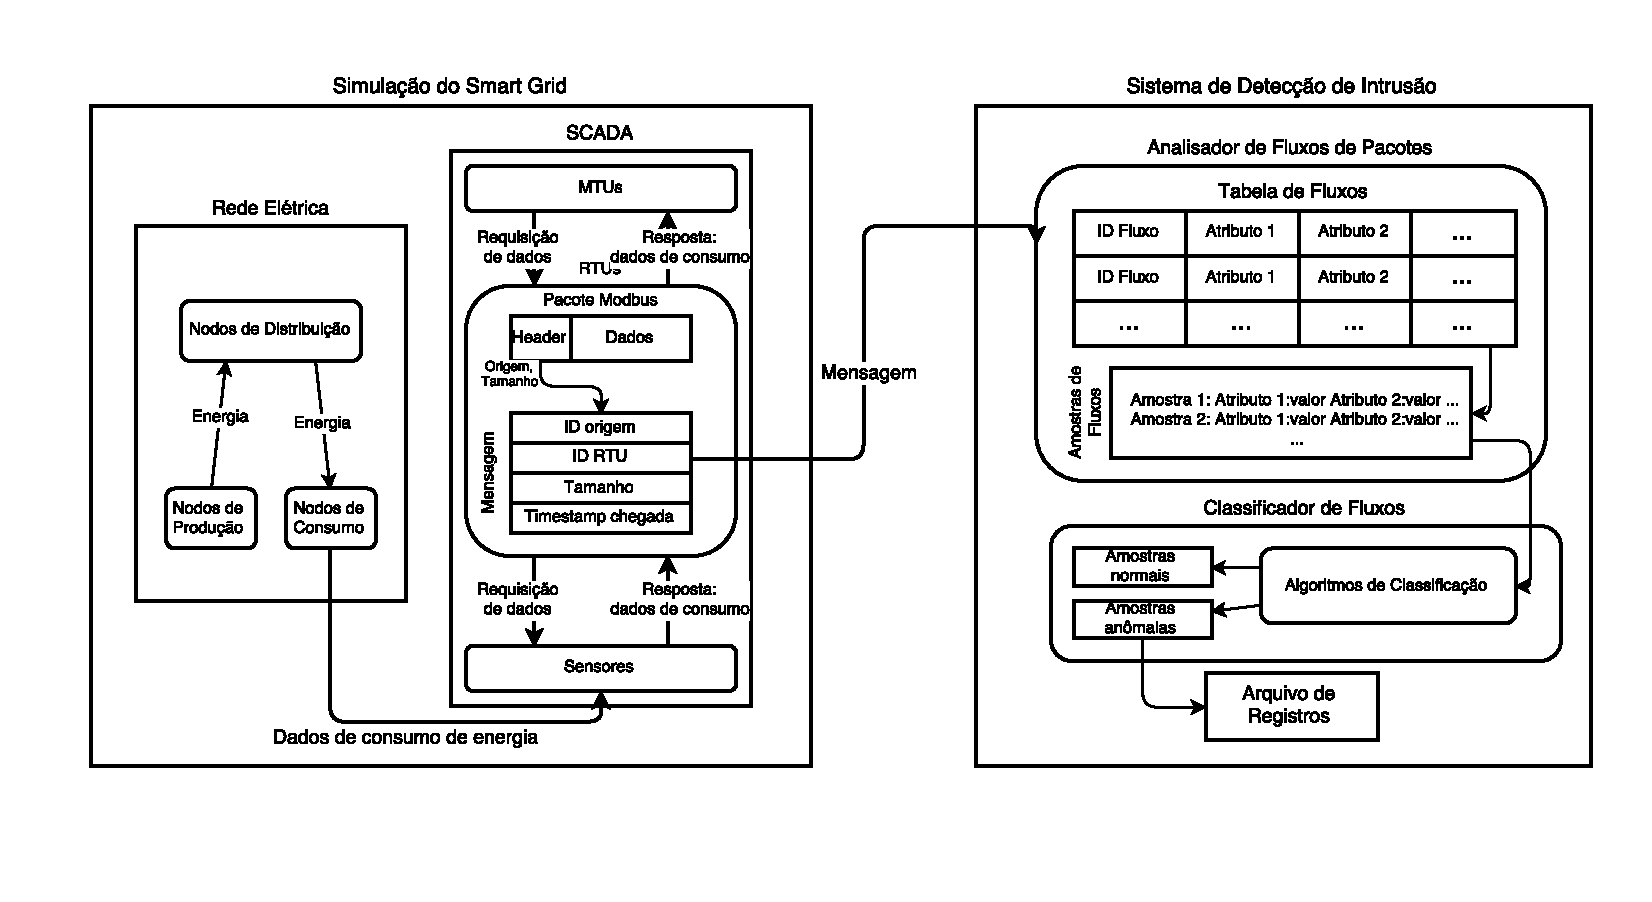
\includegraphics[width=38em]{sdi_diagram}
   \end{center}
   \label{sdi_diagram}
\end{figure}

A Figura \ref{sdi_diagram} ilustra a arquitetura conceitual do mecanismo de detecção proposto. Inicialmente, são obtidos os dados do tráfego da simulação. Todos os pacotes de dados que são enviados pelos sensores às RTUs são analisados, e são recuperados de origem, destino, tamanho e \emph{timestamp} do pacote. As informações são enviadas para o Analisador de Fluxos. O analisador recebe cada mensagem com informações de um pacote que chega ao módulo, e o insere na em duas tabelas, uma tabela de fluxos e uma tabela de amostras. Enquanto a tabela de fluxos armazena os valores computados dos atributos dos fluxos até o fim da execução, a tabela de amostras armazena amostras dos atributos dos fluxos durante um determinado período de tempo, que serão utilizadas na classificação.

Cada par de sensor de origem com RTU de destino representa um fluxo da aplicação SCADA. Para cada fluxo identificado, os seguintes atributos são armazenados:
\begin{itemize}
\item{\emph{Quantidade de Pacotes}}: Quantidade de pacotes registrados para um determinado fluxo durante toda a execução.
\item{\emph{Tamanho Médio dos Pacotes}}: Tamanho médio dos pacotes de um fluxo.  
\item{\emph{Tempo Médio de Chegada Entre Pacotes}}: Tempo médio entre a chegada ao destino de dois pacotes consecutivos em um mesmo fluxo.
\item{\emph{Tamanho Mínimo de Pacote}}: Tamanho do menor pacote registrado em um fluxo.
\item{\emph{Tamanho Máximo de Pacote}}: Tamanho do maior pacote registrado em um fluxo.
\item{\emph{Timestamp}}: Horário de chegada ao destino do último pacote registrado no fluxo.
\end{itemize}

A cada intervalo de tempo de amostragem, as amostras de fluxos são obtidas pelo Classificador de Fluxos, que utiliza algoritmos de classificação de dados para identificar amostras de tráfego normal e amostras de tráfego anômalo. Quando uma amostra de fluxo é identificada como anômala, ela é armazenada em um arquivo de registros, que documenta todas as incidencias de tráfego anormal com os dados de origem, destino, \emph{timestamp} e valores dos atributos da amostra de fluxo que foi identificada como anômala.

\section{Implementação e Análise de Resultados}
\label{secimpl}
Esta seção descreve a implementação de um protótipo do mecanismo de detecção de anomalias apresentado para a ferramenta ASTORIA, e execução dos experimentos e avaliação análise dos resultados, com o objetivo de avaliar se o mecanismo de detecção proposto é adequado para a identificação de anomalias em uma simulação de smart grid.

A Seção \ref{prototype} apresenta a implementação do protótipo e as ferramentas utilizadas. Na Seção \ref{sectionexp}, são descritos os experimentos executados para a avaliação do protótipo. Por fim, a Seção \ref{sectionresults} analisa os resultados obtidos nos experimentos.

\subsection{Implementação do Protótipo}
\label{prototype}
O framework ASTORIA foi utilizado para a simulação do ambiente smart grid e para a geração de cenários de ataques cibernéticos. No ASTORIA, as RTUs são implementadas pela classe \emph{RTU}, que gerencia os pacotes de rede recebidos dos sensores, modelados pela classe \emph{ModbusProtocol}. O envio das mensagens Das RTUs para o módulo de detecção foi implementado utilizando um \emph{socket} de rede UDP através da biblioteca \emph{sys/socket.h}. A classe \emph{FlowAnalyser} implementa o componente Analisador de Fluxos, que recebe as mensagens que chegam ao módulo de detecção, analisa os pacotes e armazena os atributos dos fluxos.

As tabelas que armazenam os valores dos atributos são definidas pela classe \emph{AttributeTable}, que implementa métodos para determinar se um fluxo já existe, obter os valores dos atributos de um fluxo e inserir valores nos atributos de um fluxo. Os valores são armazenados em um mapeamento de uma chave do tipo \emph{string}, caracterizada pelos identificadores dos nodos pertencentes a cada fluxo, com um vetor contendo os valores de cada atributo. A cada período de amostragem, as amostras da tabela são escritas em um arquivo de texto e a tabela é esvaziada. A classe \emph{FlowClassifier}, que implementa o componente Classificador de Fluxos, obtém o arquivo de amostras gerado para classificação.

O algoritmo OCSVM é utilizado na classificação das amostras. Para a implementação do OCSVM, foi utilizada a biblioteca LIBSVM \cite{libsvm}. A LIBSVM contém implementações do algoritmo SVM e suas variações, incluindo o OCSVM, e fornece \emph{scripts} para o treinamento e classificação de conjuntos de dados. A classe \emph{FlowClassifier} utiliza os \emph{scripts} da LIBSVM para  treinar o OCSVM e para classificar as amostras utilizando o algoritmo treinado.

\subsection{Execução dos Experimentos}
\label{sectionexp}
A topologia utilizada das simulações utilizadas nos experimentos, ilustrada na Figura \ref{figtopology}, é similar à topologia descrita pelos autores em \cite{wermann2015astoria}, porém com uma quantidade menor de nodos de produção e consumo, sendo composta por 1 MTU, 14 RTUs e 168 sensores.

\begin{figure}[h]
   \caption{Topologia utilizada nos experimentos}
   \begin{center}
       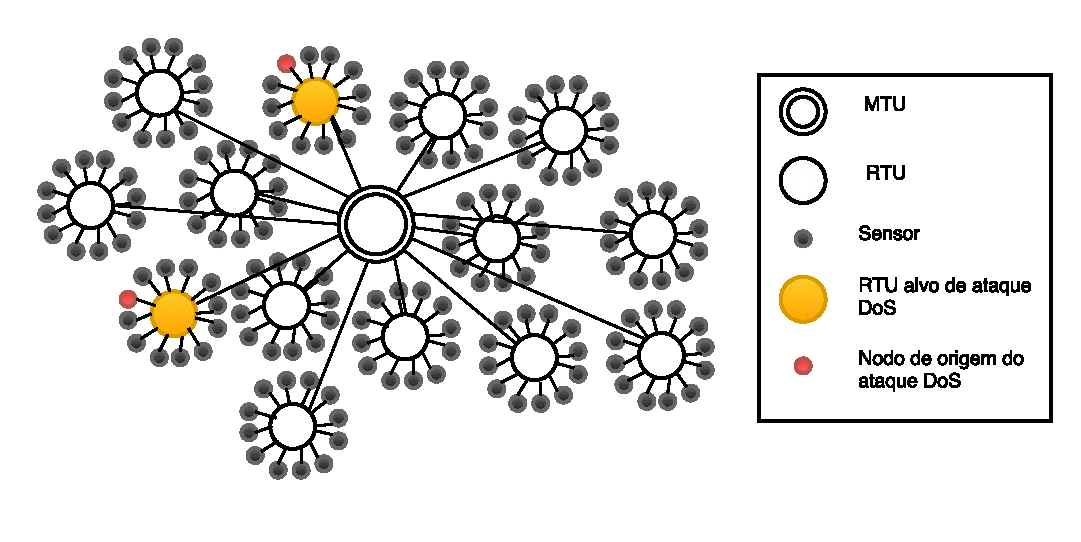
\includegraphics[width=24em]{topologia}
   \end{center}
   \label{figtopology}
\end{figure}

Na configuração das simulações, dois modelos de simulação foram utilizados, ambos com tempo total de execução de 1800 segundos e o passo de execução de 2 segundos. O primeiro modelo de simulação utiliza o tráfego puro gerado pela configuração que foi definida. No segundo modelo de simulação, atrasos aleatórios são introduzidos ao intervalo de tempo entre as requisições enviadas por algumas RTUs, causando variações nos intervalos de envio das requisições. Cada requisição enviada por uma RTU tem uma chance de 25\% de sofrer um atraso aleatório de 100, 200, 300 ou 400 milissegundos.

Para a introdução de anomalias no cenário da simulação, foi utilizado o ataque DoS fornecido pelo framework ASTORIA. Dois perfis de ataque foram utilizados no experimento, ambos com duas RTUs sendo atacadas por um de seus respectivos sensores. O primeiro perfil define um ataque de alta potência, com o intervalo de envio de pacotes variando entre 2 e 50 milissegundos, o que gera entre 20 e 500 pacotes por segundo. No segundo perfil, o ataque realizado é de baixa potência, e o intervalo de envio dos pacotes varia entre 200 e 500 milissegundos, enviando entre 2 e 5 pacotes por segundo. Para obter dados de tráfego com anomalias no tamanho dos pacotes para os experimentos, foram geradas cargas de dados com alteração nos tamanhos dos pacotes obtidos. Os conjuntos de dados gerados são semelhantes aos dados obtidos de uma simulação normal, mas com variações inseridas nos valores obtidos para o tamanho dos pacotes em alguns fluxos. Os valores anômalos inseridos incluíram pacotes com 80\%, 120\%, 200\% e 400\% do tamanho original. Os experimentos foram realizados com 30 repetições e 95\% de confiança.

\subsection{Análise dos Resultados}
\label{sectionresults}

Para a avaliação dos resultados obtidos nos experimentos, foram utilizadas as métricas Taxa de Verdadeiros Negativos (TVN),  Taxa de Falsos Negativos (TFN), Taxa de Verdadeiros Positivos (TVP), Taxa de Falsos Positivos (TFP) e Acurácia, amplamente utilizados na avaliação de sistemas de classificação \cite{nguyen2008survey}.

\begin{figure}[h]
   \caption{Resultados dos experimentos com um ataque DoS de alta potência}
   \begin{center}
       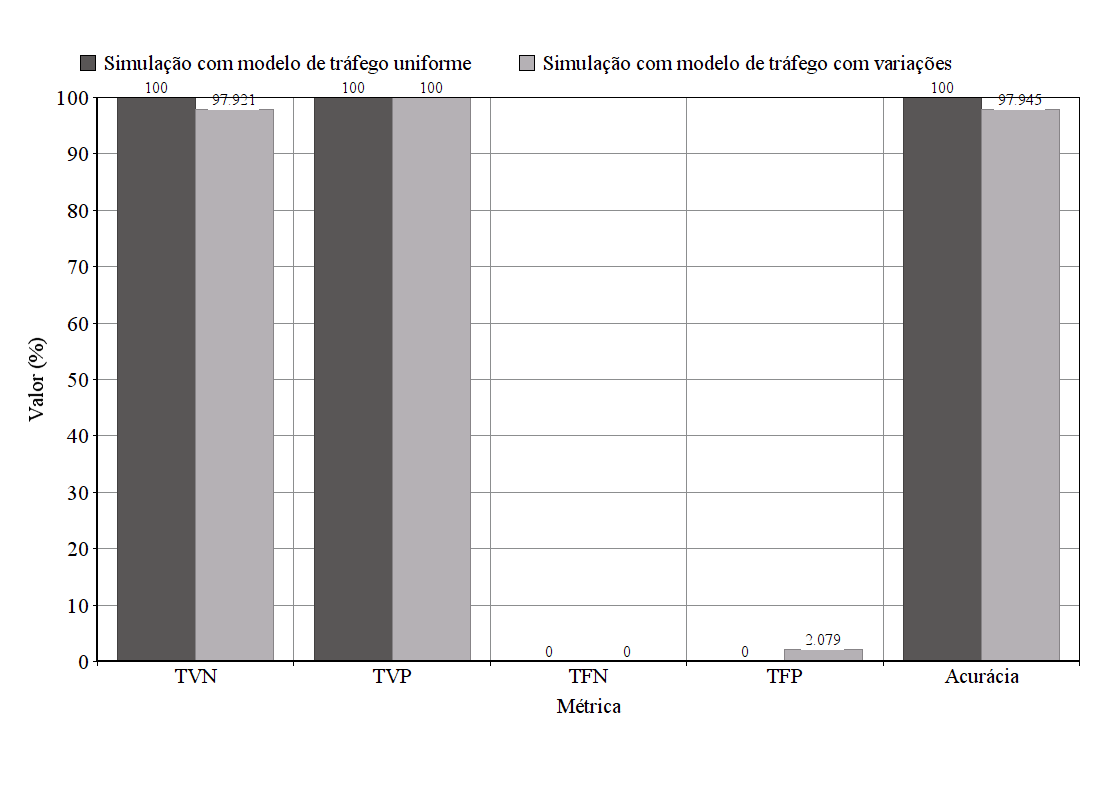
\includegraphics[width=20em]{chartdos1}
   \end{center}
   \label{chartdos1}
\end{figure}

A Figura \ref{chartdos1} apresenta os resultados obtidos na classificação do tráfego da simulação durante a ocorrência de um ataque DoS de alta potência. Primeiramente, é possível observar que, nos experimentos que utilizaram a simulação com modelo de tráfego uniforme, o sistema de detecção foi capaz de classificar corretamente todas as amostras, atingindo uma acurácia de 100\%. Já nos experimentos que utilizaram a simulação com modelo de tráfego com variações, apesar do sistema ter identificado corretamente todas as amostras de tráfego anômalo, uma parcela das amostras de fluxos normais foram classificadas como anômalas, gerando uma TFP de 2,079\%. Podemos atribuir esses resultados ao modelo de classificação que é gerado pelo algoritmo de detecção. Quando utilzamos o modelo de tráfego uniforme, o tráfego se mantém constante ao longo da execução, gerando amostras de tráfego que possuem valores de atributos iguais ou com variações muito pequenas. Quando essas amostras são utilizadas no treinamento do algoritmo, o modelo gerado para solucionar a classificação é muito simples, pois amostras de tráfego normal sempre serão iguais às amostras utilizadas no treinamento, e qualquer amostra com uma pequena variação é caracterizada como anômala. Quando o modelo de tráfego com variações é utilizado, o classificador de classe única não é capaz de incorporar toda a diversidade de dados do conjunto de treinamento ao modelo de classificação. Assim, algumas amostras com variações, provenientes de tráfego normal, são consideradas fora da classe descrita pelo modelo, e classificadas como anômalas. Ainda assim, o classificador obteve acurácia de 97,945\% na classificação do tráfego nesse cenário.

\begin{figure}[h]
   \caption{Resultados dos experimentos com um ataque DoS de baixa potência}
   \begin{center}
       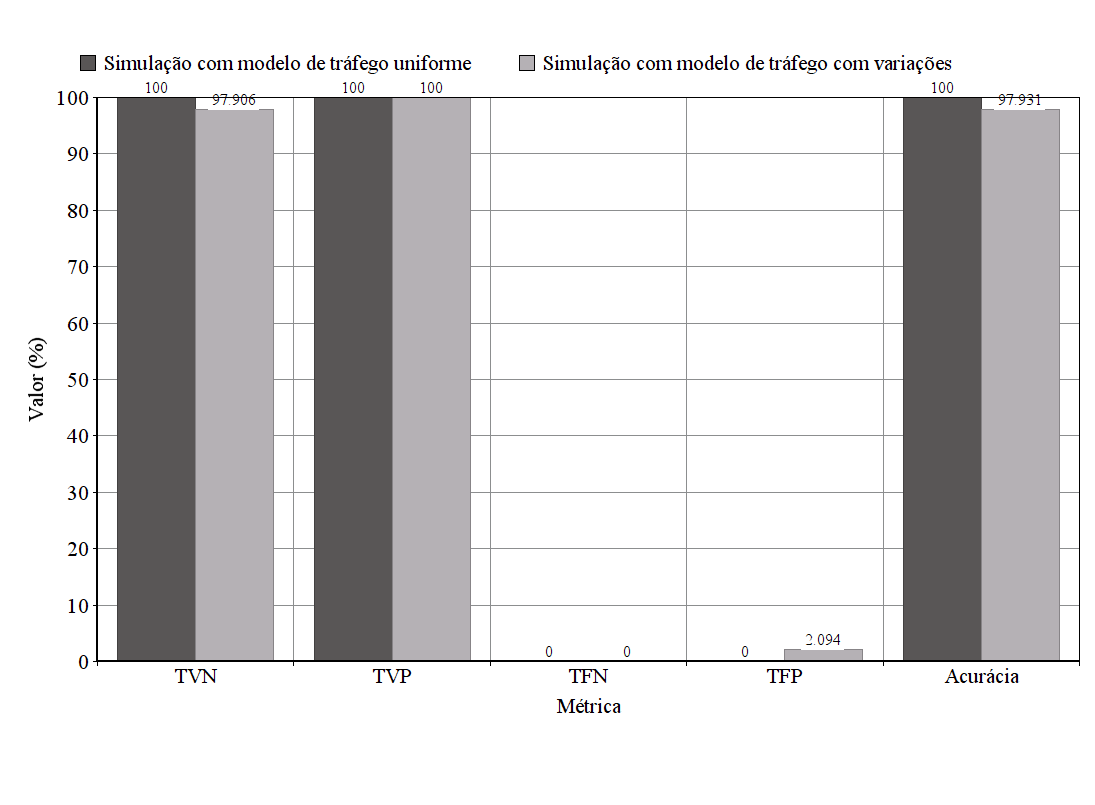
\includegraphics[width=20em]{chartdos2}
   \end{center}
   \label{chartdos2}
\end{figure}

Os resultados obtidos para a classificação do tráfego durante um ataque DoS de baixa potência são mostrados na Figura \ref{chartdos2}. Os resultados obtidos para esse cenário são semelhantes aos resultados obtidos nos cenários com o ataque DoS de alta potência. Nas execuções com a simulação de modelo uniforme de tráfego, o sistema de detecção também classificou corretamente todas as amostras, com 100\% de acurácia. Nas execuções com a simulação de modelo de tráfego com variações, as amostras de fluxos provenientes dos ataques também foram 100\% classificadas como anômalas, mas com uma TFP de 2,094\%, obtendo 97,931\% de acurácia. Da mesma forma que nos experimentos com o ataque de alta potência, o modelo de classificação gerado a partir da simulação de tráfego com variações não compreendeu toda a diversidade de dados descrita pelas amostras de tráfego. Desse modo, apesar das anomalias geradas serem mais próximas do tráfego normal, o classificador excluiu as amostras anômalas da classe normal da mesma forma que excluiu parte das amostras normais que possuíam variações.

\begin{figure}[h]
   \caption{Resultados dos experimentos com inserção de anomalias no tamanho dos pacotes}
   \begin{center}
       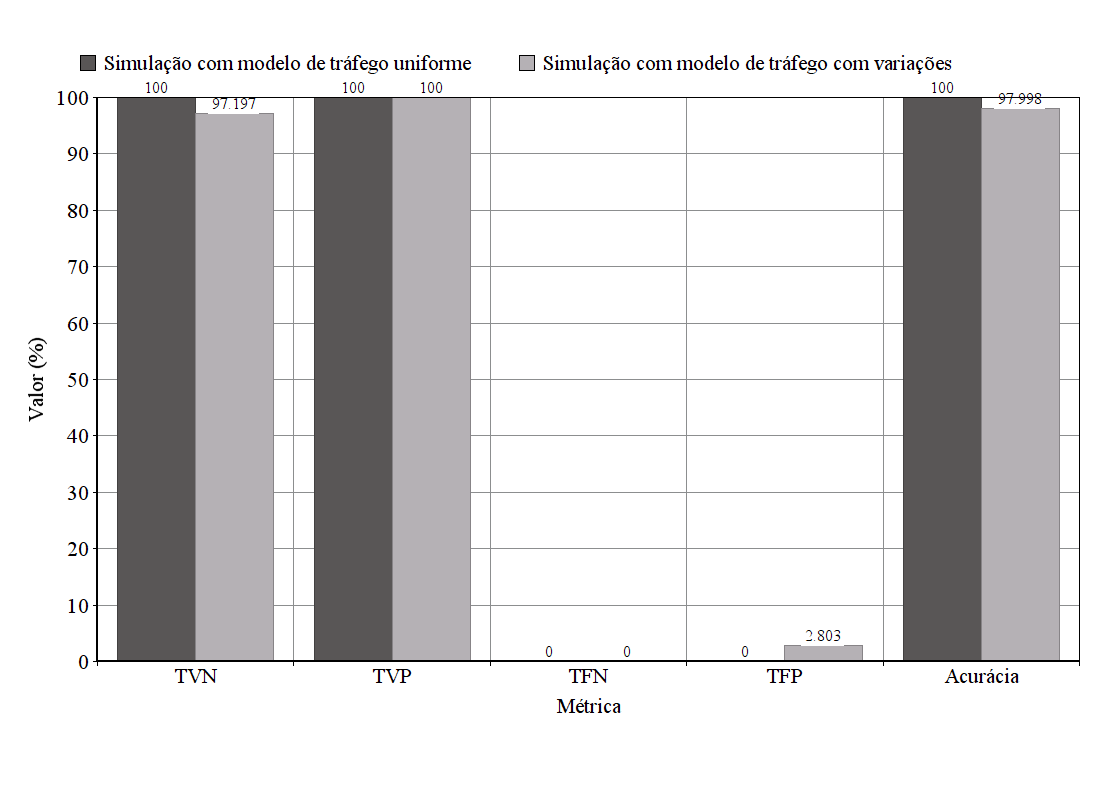
\includegraphics[width=20em]{chartsize}
   \end{center}
   \label{chartsize}
\end{figure}

Por fim, a Figura \ref{chartsize} apresenta os resultados obtidos para a classificação do tráfego utilizando cargas de dados com anomalias no tamanho dos pacotes. Os resultados seguiram o mesmo comportamento dos experimentos com os cenários de ataques DoS. As execuções utilizando a simulação com o modelo de tráfego uniforme obtiveram acurácia de 100\% na classificação. As execuções utilizando a simulação com modelo de tráfego com variação identificaram todas as amostras anômalas corretamente, porém com uma TFP de 2,803\%, atingindo 97,998\% de acurácia.

A partir dos resultados apresentados, podemos constatar que o classificador obtém resultados mais precisos para a classificação de tráfegos mais estáveis, com maior uniformidade nos dados e poucas variações. Quando pequenas variações são inseridas no tráfego, o modelo de classificação gerado passa a não assimilar toda a diversidade de dados presente no conjunto de treinamento, e falsos negativos passam a ocorrer na classificação. Todavia, a TFN foi zero em todos os experimentos, indicando que todas as ocorrências de tráfego anômalo foram identificadas, e a acurácia superou 97\% em todas as execuções. Esses resultados apontam que sistemas de detecção de anomalias baseados no algoritmo OCSVM são viáveis em estruturas de comunicação de smart grids.

Para aumentar a precisão do sistema, seria possível complementar o algoritmo de detecção de anomalias com técnicas de \emph{Signature Based Detection} utilizando perfis de ataques para a detecção, como utilizado em \cite{yang2013iecdetection}. Para isso, seria necessário ter acesso a dados sobre ataques conhecidos a smart grids, e sobre o comportamento do tráfego da rede durante a ocorrência de ataques. Outra possibilidade seria utilizar na classificação um algoritmo de classificação em duas classes, como o SVM tradicional. Nesse caso, o conjunto de treinamento seria composto por uma classe positiva, representada por amostras de tráfego normal, e uma classe negativa, representada por amostras de tráfego em cenários de ataques ou anomalias.

\section{Trabalhos Relacionados}
\label{related}
Sistemas de Detecção de Intrusão (SDIs) baseados em detecção de anomalias para sistemas SCADA são apresentados em \cite{coutinho2009anomaly} e \cite{tsang2005multi}.
SDIs baseados em \emph{Signature Based Detection} são apresentados em \cite{carcano2011multidim}, que apresenta um SDI para sistemas SCADA que utiliza modelagem e análise de estados, \cite{yang2013iecdetection}, que apresenta um IDS baseado em perfis de ataques para sistemas SCADA que utilizam o protocolo IEC 60870-5-104, em \cite{2014multiattribute}, que descreve um framework distribuído para a detecção de intrusão, e em \cite{2014temporalintrusion}, em que um IDS específico para sistemas SCADA é proposto baseado na identificação de relações de tempo entre os pacotes da rede.
IDSs para AMIs são propostos em \cite{aliprobabilistic}, utilizando dados coletados da AMI e modelando seu comportamento para comparação com especificações de configuração dos dispositivos, e em \cite{mclaughlinamids}, que apresenta o framework AMIDS, que utiliza registros de medição com dados de consumo para modelar o comportamento do AMI.

\section{Conclusão e Trabalhos Futuros}
\label{capconcl}
O desenvolvimento dos smart grids possibilita o consumo e distribuição mais eficientes da energia elétrica, a utilização de fontes renováveis de energia e abre diversas possibilidades para a utilização de novas tecnologias, a fim de tornar o sistema de distribuição mais seguro e confiável. No entanto, smart grids são suscetíveis a diversos ataques, tanto aos componentes da rede elétrica quanto aos componentes da rede de comunicação, tornando desenvolvimento de mecanismos para garantir a segurança dos smart grids de grande importância.

Neste trabalho, propusemos um sistema de detecção de anomalias para uma ferramenta de simulação de smart grid. A ferramenta de simulação utilizada foi o framework ASTORIA, capaz de definir ataques sobre a simulação de um smart grid. O sistema de detecção desenvolvido utiliza as informações do tráfego da simulação para identificar anomalias através da classificação dos dados. O sistema calcula os atributos dos fluxos da rede, que são classificados utilizando o algoritmo \emph{One-Class Support Vector Machine}, de classificação em classe única. O algoritmo foi treinado utilizando amostras de tráfego normal da simulação, a fim de diferenciar tráfego normal de tráfego anômalo apenas com o conhecimento do tráfego normal da rede. O sistema de detecção foi avaliado através de experimentos que utilizaram cenários com ataques DoS de maior intensidade e de menor intensidade, além de cenários com anomalias no tamanho medido para os pacotes. Os resultados dos experimentos demonstraram que o sistema de detecção de anomalias desenvolvido é capaz de identificar corretamente a ocorrência de ataques e anomalias de intensidades variadas à rede, apesar de apresentar uma pequena taxa de ocorrência alarmes falsos quando o tráfego sendo analisado apresenta uma quantidade maior de variações.

Como trabalhos futuros, propomos avaliar o desempenho do sistema de detecção utilizando outros algoritmos de classificação em classe única, como o \emph{Support Vector Data Description} \cite{tax2004support} e o \emph{Kernel Principal Component Analisys} \cite{hoffmann2007kernel}. Também propomos melhorar a acurácia do sistema de detecção combinando o algoritmo de classificação em classe única com técnicas de detecção baseadas em assinatura, como as utilizadas em \cite{yang2013iecdetection}, utilizando perfis que descrevam ataques comuns a sistemas SCADA, a fim de diminuir a quantidade de alarmes falsos e aumentar a precisão da detecção.


\bibliographystyle{sbc}
\bibliography{sbc-template}

\end{document}
